% Background

% Main chapter title
%\chapter[toc version]{doc version}
\chapter{Background}

% Short version of the title for the header
%\chaptermark{version for header}

% Chapter Label
% For referencing this chapter elsewhere, use \ref{ChapterTemplate}
\label{Background}

This chapter will cover the concepts needed to contextualize and understand the \ac{ucttp} and the algorithms used to obtain the final result, namely the \ac{mcts} and \ac{hc} algorithms.

%\section Terminology

\section{Combinatorial Optimization Problems}

Finding a solution for maximizing or minimizing a value is common in several real world problems. These problems often require searching for an optimal solution from a finite set of possibilities. They are characterized by their discrete nature and the challenge of finding optimal solutions in large search spaces.

\acp{cop} arise in various fields, such as artificial intelligence, machine learning, auction theory, applied mathematics, and so on. Some well-known \acp{cop} include Knapsack Problem, Traveling Salesman Problem, and Graph Coloring. 

To solve these problems, various algorithmic techniques are used, including:
\begin{itemize}
\item \textbf{Exact algorithms:} Guarantee optimal solutions by exhaustively exploring the solution space. However, they can be computationally expensive, especially for large and complex problems, because their complexity often grows exponentially.
\item \textbf{Approximation algorithms:} Produce provably near-optimal solutions, providing a quantifiable measure of how far the solution might diverge from the best possible one, making them valuable for problems where exact solutions are infeasible.
\item \textbf{Heuristic algorithms:} Focus on practicality and efficiency by finding good solutions within a reasonable time frame. While they do not ensure optimality, they are often effective for solving large-scale problems. This type of algorithms will be the primary focus of this dissertation.
\end{itemize}

\section{University Course Timetabling Problem}

\ac{ucttp} is a NP-hard \ac{cop} that involves allocating events, rooms, lecturers, and students to weekly schedules while meeting certain predefined constraints. It falls under the broader category of Educational Timetabling, which also includes other challenging problems such as Examination Timetabling. 

Due to the size and complexity of the problem, obtaining an optimal solution in usable time is typically infeasible. Therefore, it is necessary to employ robust optimization techniques.

\subsection{Curriculum-Based and Post-Enrollment Course Timetabling}

\ac{ucttp} can be categorized into two main types:

\begin{itemize}
\item \textbf{Curriculum-Based Course Timetabling (CB-CTT):} Courses are grouped into predefined curricula, ensuring that no student or lecturer is allocated to overlapping courses within their curriculum.

\item \textbf{\ac{pe-ctt}:} Events are scheduled after students enroll in their courses, taking into account their preferred event combinations while minimizing conflicts.
\end{itemize}

These two problems differ significantly in terms of timing, flexibility, and constraints. \ac{pe-ctt} is performed after the student has enrolled in their courses, while \ac{cb-ctt} is performed first. \ac{pe-ctt} adjusts to the student choices, providing greater flexibility, while \ac{cb-ctt} follows a more rigid and predefined structure. Furthermore, \ac{pe-ctt} often involves more complex constraints due to diverse student preferences, whereas \ac{cb-ctt} deals with more predictable patterns. As a result, \ac{pe-ctt} is appropriate for institutions with a flexible course enrollment, while \ac{cb-ctt} is ideal for institutions with fixed curricula. \ac{fcup}'s timetables generation fits into \ac{cb-ctt}.

\subsection{Constraints}
%How can a university/school schedule its classes to make the best use of teachers and classrooms without conflicts?
In the context of \ac{ucttp}, constraints are often divided into two different types:
\begin{itemize}
\item \textbf{Hard constraints:} Ensure the feasibility of the timetable and must be strictly satisfied. Typically, a hard constraint includes avoiding overlapping events for the same student or a lecturer. 
\item \textbf{Soft constraints:} Represent preferences to improve the quality of the solution without being mandatory. An example of a soft constraint is minimizing gaps in students' timetables to ensure a more compact timetable.
\end{itemize}

\section{International Timetabling Competition (ITC)}

Since 2002, the \ac{patat}\footnote{\url{https://patatconference.org/communityService.html}} has supported timetabling competitions to encourage research in this field. There have already been five editions of the \ac{itc}, with three focusing on university timetabling. The third edition, held in 2011, centered on high school timetabling.

The first \ac{itc} in 2002 focused on the \ac{pe-ctt} problem and utilized artificially generated instances. Over successive editions, the competition introduced problem instances that increasingly reflected real-world constraints and complexities.

The \ac{itc-2007}\footnote{https://www.eeecs.qub.ac.uk/itc2007/} was structured into three distinct tracks: Examination Timetabling Problem, Post-enrollment Course Timetabling, and Curriculum-based Course Timetabling. The second one is an extended version of the previous competition. This dissertation focuses on the Curriculum-Based Course Timetabling track (track 3) of the \ac{itc-2007}, as it aligns with the problem under investigation. Even after 18 years, these benchmark datasets remain widely used in academic research and optimization studies, demonstrating their relevance in the field.

\section{Monte Carlo Tree Search}

\ac{mcts} is a decision-making algorithm that has been successfully applied in a variety of optimization problems with a huge search space. The algorithm has proven to be particularly effective in games such as Go and Chess, where the algorithm can even outperform the best human players.

\subsection{Phases}
%TODO \cite{browne_survey_2012}

\begin{figure}
      \centering
      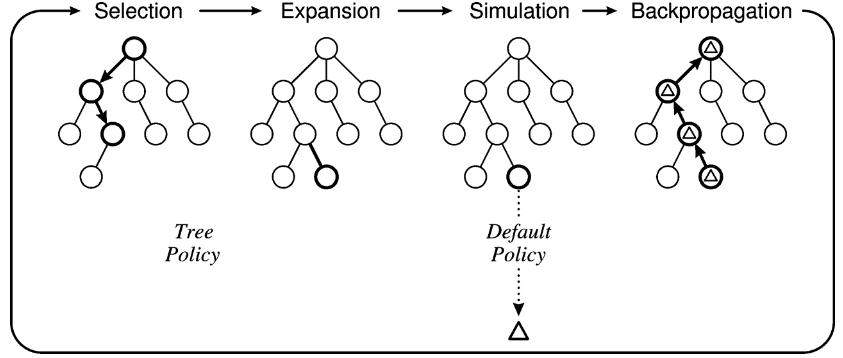
\includegraphics[width=0.7\columnwidth]{Background/MCTS_approach.png}
      \caption[MCTS approach]
      {One MCTS iteration \cite{browne_survey_2012}}
      \label{fig:mcts_approach}
\end{figure}

The algorithm consists of four phases, as illustrated in Figure \ref{fig:mcts_approach}  \cite{browne_survey_2012}. These phases are repeated for a predefined number of iterations or until a computational budget (such as time or memory) is reached. The phases are as follows:

\begin{enumerate}
	\item \textbf{Selection:} The tree is traversed from the root node until it finds a node that is not completely expanded, i.e., a non-terminal node with unvisited children. The selection is guided by a policy that balances exploration and exploitation. Typically, the policy used is \ac{uct}, which selects nodes that maximize formula \ref{uct_formula}.
	 
	\begin{equation}
	UCT = \frac{w_i}{n_i} + 2C\sqrt{\frac{2\ln{n}}{n_i}},\label{uct_formula}
	\end{equation} where \(w_i\) is the total reward of all playouts through this state, \(n_i\) is the number of visits of child node \(i\), \(C\) is a constant greater than zero (typically \(\sqrt{2}\)), and \(n\) is the number of visits of the parent node.
    \item \textbf{Expansion:} One or more child nodes are added to the node previously reached in the selection phase.
    \item \textbf{Simulation:} From the newly added node(s), a simulation is performed according to a default policy, which may include random moves until a terminal node is reached.
    \item \textbf{Backpropagation:} The simulation result is then propagated back through the traversed nodes, where the number of visits and the average reward for each node are updated until it reaches the root.
\end{enumerate}

\section{Local Search}

Local search is an optimization technique that iteratively improves a solution within a given search space by making small changes and retaining those that yield better results. It is effective for large-scale problems where the search is computationally expensive or unfeasible. Popular local search algorithms include \ac{hc}, \ac{sa}, \ac{ts}, and Genetic Algorithms (GA). While local search algorithms are powerful, they can sometimes get stuck and fail to find the global best solution. Techniques such as simulated annealing help escape local optima and explore a broader range of solutions.

\subsection{Hill Climbing}

\ac{hc} is a local search optimization algorithm that begins with an initial solution, which can be randomly generated or specifically chosen depending on the problem. From this starting point, \ac{hc} evaluates neighbouring solutions, which are generated by making small modifications to the current solution. If a neighbouring solution is found to be better than the current one, the algorithm moves to that new solution. The algorithm finishes when there is no better neighbouring solution that offers an improvement over the current one, indicating that a local optimum has been attained. 

While \ac{hc} is effective and easy to implement, it has limitations.The algorithm can get stuck in:

\begin{itemize}
\item \textbf{Local optimum:} A solution state that is better than its neighbours but not necessarily the global optimum, i.e., the best possible solution in the entire search space, restricting further improvement.
\item \textbf{Plateaus:} Mostly flat regions in the search space where neighbouring solutions have the same value, making it challenging for the algorithm to determine a direction of improvement.
\item \textbf{Ridges:} A region in the search space where moving in all directions appears to lead downhill, and reaching a better solution often requires a sequence of non-improving moves, which \ac{hc} does not explore.
\end{itemize}

To address these issues, variations of the algorithm have been developed:

\begin{itemize}
\item \textbf{Simple Hill-Climbing:} Evaluates one neighbour at a time and moves to the first improvement found, making it efficient but susceptible to local maxima.
\item \textbf{Steepest-Ascent Hill-Climbing:} Evaluates all neighbours of the current state and chooses the best among them. This algorithm is a variation of the simple hill-climbing algorithm but takes more time.
\item \textbf{Stochastic Hill-Climbing}: Randomly selects a neighbour, without evaluation, and moves to it if it improves the solution. This approach is less commonly used than the other two.
\end{itemize}

\section{Previous Work}

\begin{figure}
      \centering
      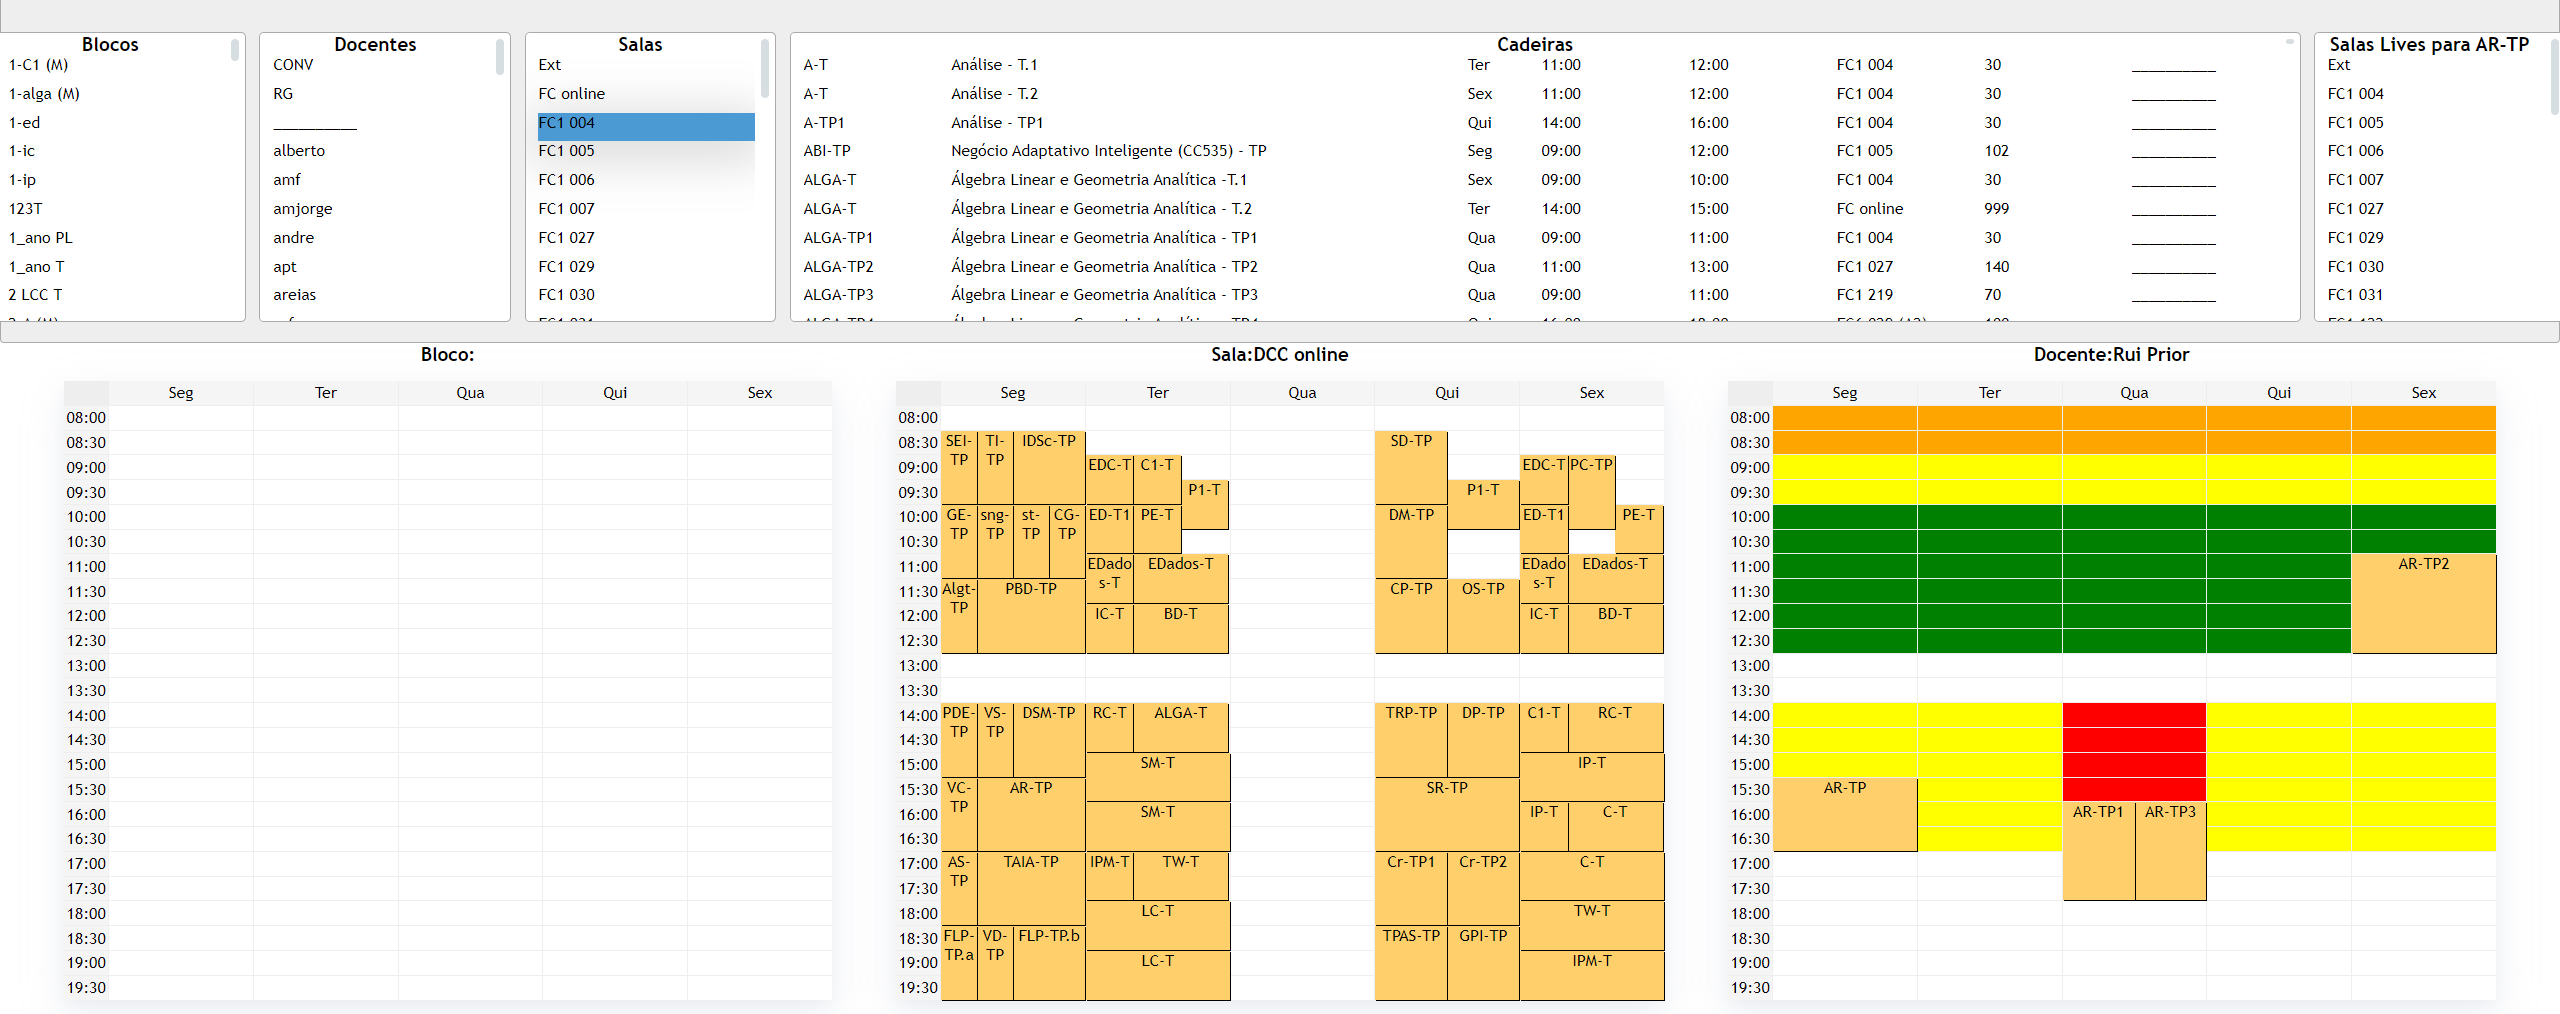
\includegraphics[width=1.0\columnwidth]{Background/previous_work.png}
      \caption[Previous work interface]
      {Previous work interface}
      \label{fig:previous_work_interface}
\end{figure}

\begin{figure}
      \centering
      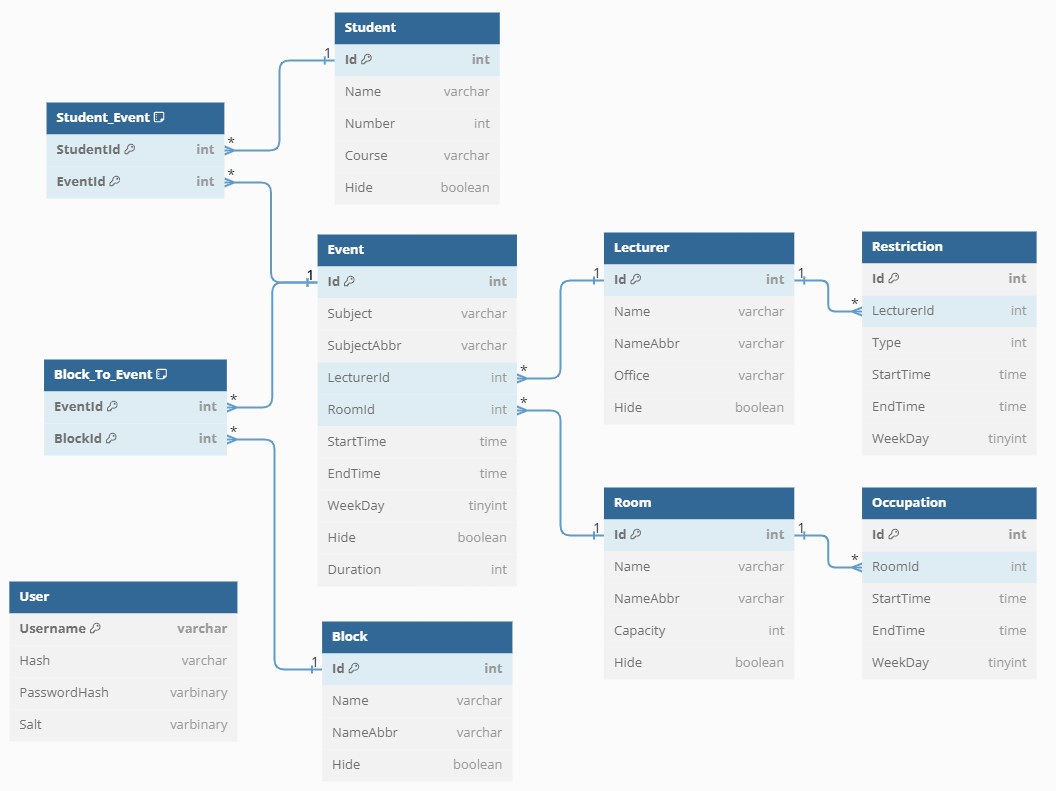
\includegraphics[width=1.0\columnwidth]{Background/uml.png}
      \caption[Previous work UML]
      {Previous work UML}
      \label{fig:previous_work_uml}
\end{figure}

A previous project\footnote{\textbf{Front-end:} \url{https://github.com/luismdsleite/schedule} \textbf{Back-end:} \url{https://github.com/luismdsleite/schedule-backend/tree/main}} developed a timetabling visualization tool using Flask and reactive programming principles with the Elm language. Flask facilitated data management and communication between the front-end and the database (Figure \ref{fig:previous_work_uml}), ensuring that timetable updates were efficiently processed and displayed. 

This tool allow users to manually construct and modify schedules while providing a responsive interface (Figure \ref{fig:previous_work_interface}). However, despite its usability, the tool has some limitations that this dissertation attempts to address:

\begin{itemize}
\item \textbf{No conflict detection support:} Users had to manually check for conflicts, increasing the risk of errors.
\item \textbf{Lack of automated guidance:} It did not provide recommendations or suggestions to help users make optimal scheduling decisions.
\item \textbf{No quality assessment:} The system lacked mechanisms to evaluate the quality of a given timetable.
\end{itemize}

%\subsection{Reactive Programming}

%\subsubsection{Elm}


